\documentclass[12pt, letterpaper]{article}

%\usepackage[margin=1in]{geometry}
%\usepackage{enumitem}
%\usepackage{float}
%\usepackage{empheq}
%\usepackage{datetime}

\usepackage[shortlabels]{enumitem}
\usepackage{empheq}
\usepackage{url}
\usepackage{amsmath, amssymb}
\usepackage[export]{adjustbox} % also loads graphicx
\usepackage{textcomp}
\usepackage{color}
\usepackage{nicefrac}
\usepackage{cancel} % \cancel for strike through text but diagonal
\usepackage[normalem]{ulem} % for \sout strike through text

%\usepackage{steinmetz}
%\newcommand{\HW}{Hot Wheels\textsuperscript{\textregistered}}
\newcommand{\HW}{Hot Wheels}
%\newcommand{\Matchbox}{Matchbox\textsuperscript{\textregistered}}
\newcommand{\Matchbox}{Matchbox}

\newcommand{\revise}[1]{{\color{red}\textit{#1}}}
\newcommand*{\multicitedelim}{:}

\newcommand{\degree}{$^{\circ}$}
\newcommand{\degre}{^{\circ}}

\newcommand{\Ohm}{$\Omega$}

\newcommand{\Fbox}[1]{\fbox{$\displaystyle #1$}}

\newcommand{\ezfig}[2]{
\begin{figure}[t]
\centering
\includegraphics[width=\linewidth]{images/#1.png}
\caption{\label{fig:#1} #2}
\end{figure}
}

\newcommand{\ezfigstar}[2]{
\begin{figure*}[t]
\centering
\includegraphics[width=\linewidth]{images/#1.png}
\caption{\label{fig:#1} #2}
\end{figure*}
}

\newcommand{\code}[1]{{\fontfamily{pcr}\selectfont #1}}


\begin{document}
\section{Part 1: Identifying the System}
What is our system? How do we want to model it? These are the first questions to answer before writing any MATLAB code. 

\begin{figure}[t]
\centering
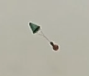
\includegraphics[width=0.5\linewidth]{images/BallMidFlight.png}
\caption{\label{fig:BallMidFlight} A photograph of our system. The system consists of a projectile traveling on an arc through the air after being thrown with some initial velocity. A drogue chute has been attached with the intention of linearly varying the aerodynamic drag, though it may have more dynamic impacts than intended.}
\end{figure}

\begin{figure}[t]
\centering
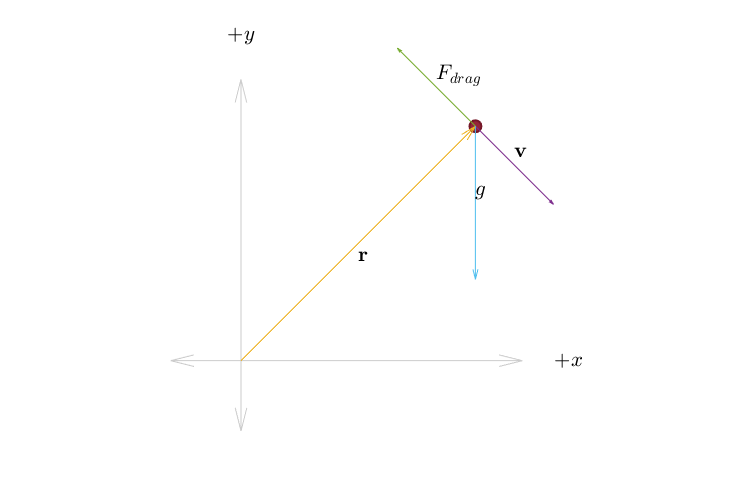
\includegraphics[width=\linewidth]{images/freebody1.png}
\caption{\label{fig:freebody1} Freebody diagram of our system showing the ball, the forces acting on it, it's velocity, and it's position in the coordinate frame.}
\end{figure}

A photograph of the system is presented in Fig.~\ref{fig:BallMidFlight}. A good first step in deriving a mathematical model of the system is to identify all the forces present on the object and draw a free body diagram. Such a diagram is presented in Fig.~\ref{fig:freebody1}. There are 2 forces I can identify that would impact the motion of the ball: gravity and air resistance. I'd also like to point out how this model does \textit{not} address the chute at all. On an ideal throw, the chute tends to trail somewhat in line with the velocity vector. This model assumes that the chute can be approximated as a constant scaling factor on the ball's inherent drag coefficient. 

But before we proceed with this 2-force model, let's remember that all models are wrong.\footnote{By stating that "all models are wrong" I'm trying to emphasize that we are always making some sort of compromise in accuracy when we decide on our model complexity. We shouldn't immediately assume that just because air resistance exists means we need to model it. We can start with a simpler model and prove that the more complicated model is justified.} I would like to start by implementing the simple parabolic model with negligible air resistance. In this model, the only force acting on the ball is gravity. 
\begin{align*}
F = F_{gravity} = mg
\end{align*}
where $g \approx 9.81\ m/s^2$.\footnote{\href{https://www.youtube.com/watch?v=7knY1U-ysY4}{https://www.youtube.com/watch?v=7knY1U-ysY4}} By application of Newton's 2nd Law,
\begin{align*}
F = ma = mg \\
\Rightarrow a = g
\end{align*}
We can rewrite this in a vector notation and solve for acceleration:
\begin{align*}
m\ddot{\bf r} &= -mg\hat{y} \\
\Rightarrow \ddot{\bf r} &= -g\hat{y}
\end{align*}
and integrate with respect to time to find velocity and position.\footnote{I have no idea if this math is right.}
\begin{align*}
\ddot{\bf r} &= -g\hat{y} \\
\int \ddot{\bf r}\ dt &= \int -g\hat{y}\ dt \\
\dot{\bf r}(t) &= -g\hat{y}t + \dot{\bf r}_0 \\
\int \dot{\bf r}(t)\ dt &= \int -g\hat{y}t + \dot{\bf r}_0\ dt \\
{\bf r}(t) &= -\frac12g\hat{y}t^2 + \dot{\bf r}_0t + {\bf r}_0
\end{align*}
The main function we need to know is the position so that we can compute its position in the \textit{future} with constant constant time complexity. (In contrast to running numerical integration to compute the position.) We should plan to have the code return functions for the velocity and acceleration as well so that we don't have to recompute it later on. That is to say, the output of our model is 
\begin{align*}
Model Output =
\begin{cases} 
\dot{\ddot{\bf r}}(t) & acceleration \\
\ddot{\bf r}(t) & velocity \\
{\bf r}(t) & position
\end{cases}
= 
\begin{cases}
-g\hat{y} \\
-g\hat{y}t + \dot{\bf r}_0 \\
-\frac12g\hat{y}t^2 + \dot{\bf r}_0t + {\bf r}_0
\end{cases}
\end{align*}
This may seem like overkill at this point in time, but it should make it easy to change the complexity in the future. 

Now we have to talk about code syntax and coordinate frames. We could represent the position as entirely independent component functions, or functions that return the quantities as vectors. If they're vectors, they could be row vectors, column vectors, or complex numbers. All of these are equivalent, but may make certain future operations easier to implement. 

The decision feels fairly arbitrary, but I feel like having the functions return column vectors would make it easier to align the code with the LaTeX.\footnote{Maybe we could return the derivatives as well as a 3x3 matrix?}\footnote{We may add a drag force to this model.}

We should also take note of what the model parameters are. We obviously have time, but there's also gravity, initial velocity, and initial position. I'll define gravity to be a constant $9.81\ m/s^2$, time will be $t \in \mathbb{R}$, and the initial velocity and initial positions will be column vectors.\footnote{We may want to make t only defined on the interval (0,impact)}\footnote{I'm going to define them in column vectors to match the functions, but we could also think about specifying them in other coordinate systems like polar coordinates if that's desired. That could be a standalone function to convert from polar to Cartesian.} 

\section{Plotting the Model}
We've made a simple model of the trajectory and it would be good to see what it looks like. You can probably plot the position components over time pretty easily with the command window, but we're going to generate these plots a lot during the course of development so let's write a function to do it for us. 

We're clearly going to want to plot the position over time, but first let's consider what would be a useful way to display the model in general. Some information to include:
\begin{itemize}
\item Kinematics Graphs
\begin{itemize}
\item Position
\item Velocity
\item Acceleration
\end{itemize}
\item Model Parameters
\begin{itemize}
\item Initial Position
\item Initial Velocity
\end{itemize}
\item Additional Info
\begin{itemize}
\item Test Number/Filename
\end{itemize} 
\end{itemize}
For now, let's address plotting the kinematics. There are plenty of different ways to do this, but I like a 3x3 grid that shows the components separately. One thing to keep in mind when creating the figure is that we're going to want to also plot the sampled data on here as well.










\end{document}